\chapter{Container-Runtimes}
\label{chap:compCtnrRuntimes}

Container-Runtimes sind das Herz eines jeden Container-Angebots. Sie instanziieren übergebene Prozesse in isolierten Containern. In diesem Kapitel werden verschiedene Runtimes miteinander verglichen und veranschaulicht, wie Runtimes neben Docker für spezielle Anforderungen besser geeignet sind.

\section{Vorgehen}
\label{sec:vorgehen}
Um verschiedene Runtimes zu vergleichen wurde eine eigene Anwendung mit drei Microservices implementiert. Dabei wurden, wie in \fref{fig:todosStack} zu sehen, verschiedene Technologien verwendet, um zu prüfen, wie die getesteten Container-Runtimes mit diesen umgehen. Diese wurde im Folgenden mit verschiedenen Runtimes bereitgestellt.

\begin{figure}[h]
	\begin{center}
		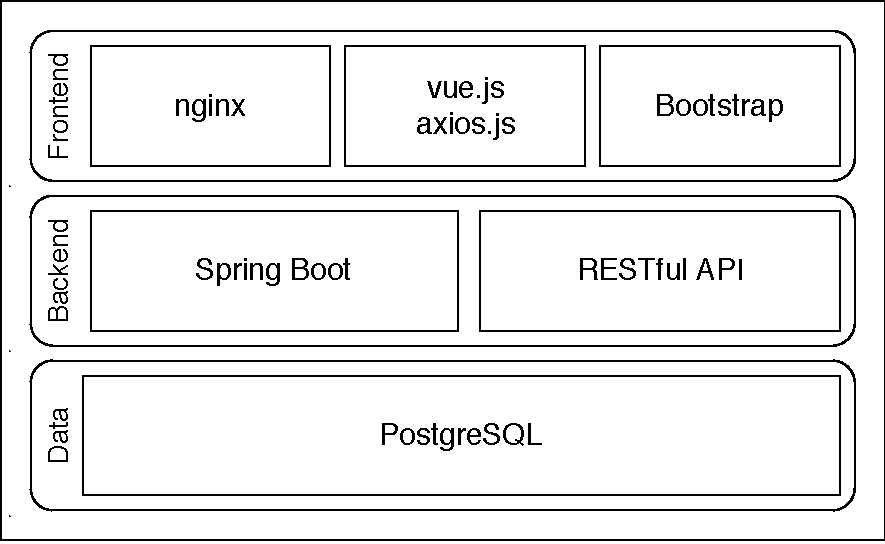
\includegraphics[width=0.7\textwidth]{bilder/microservice-example-stack.pdf}
		\caption{Beispielhafte Darstellung einer Micorservice-Architektur}
		\label{fig:todosStack}
	\end{center}
\end{figure}

\section{Docker Stack}
\label{sec:compDocker}
Docker ist der De-Facto-Standard unter den Container-Technologien und bietet eine vollständige Plattform zur Verwaltung und Orchestrierung von Container (Docker Swarm), der Verbreitung von \glspl{gls-image} (Docker Hub bzw. Docker Store) und der Verwaltung des Container-Lifecycles (Docker CLI) an.

\begin{figure}[h]
	\begin{center}
		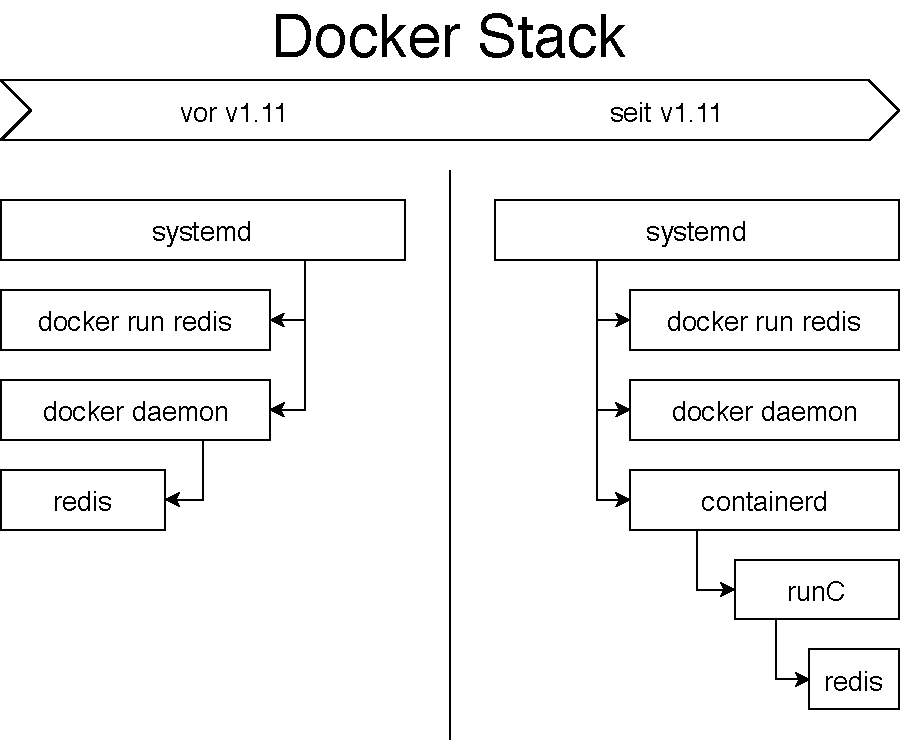
\includegraphics[width=0.9\textwidth]{bilder/docker-stack-containerd-runc.pdf}
		\caption{Docker Stack}
		\label{fig:dockerStack}		
	\end{center}
\end{figure}

Dabei kommen innerhalb des Docker Stacks die Runtimes \texttt{runc} und \texttt{containerd} zum Einsatz. Durch die in \fref{fig:dockerStack} gezeigte Abkapselung der Runtime kann Docker auf jede beliebige \gls{acr-oci}-konforme Runtime aufbauen. Der dadurch gewonnene Vorteil der Kompatibilität bietet allerdings auch Nachteile. Falls einer der vielen Komponenten im Container-Stack einen Bug aufweist, ist das Debugging der Anwendung deutlich komplexer und Fehler können langsamer gefunden werden. Zudem benötigt der Docker-Daemon privilegierte Berechtigungen um die in \fref{sec:funktionsweise} beschriebenen Konzepte zu Nutzen. Da der Daemon auch für den Download und Bau-Prozess der Images zuständig ist, werden alle Images in Docker im Kontext des Users \texttt{root} erstellt.

Notes:
\begin{itemize}
	\item Docker hub / Docker Store einfach zu nutzen
	\item gedacht für Apps
	\item großes Angebot an Images (Hub)
	\item Docker compose
	\item kein extra Tooling
	\item Netzwerk offen, einfach für Testen, unsicherer
\end{itemize}

\section{rkt}
\label{sec:compRkt}
Notes
\begin{itemize}
	\item unixesque CLI
	\item kein Zentraler Deamon, dadurch integrierbar in init system
	\item gedacht um einzelne Apps zu deployen, nicht ganze Linux Systeme
	\item kaum bis kein wissen über Kernel notwendig
	\item AppC Standard, Docker images, OCI bundles
	\item CNI Networking, CNCF Standard
	\item Secure, crypto validierung default
	\item Jedes Images SOLLTE signiert sein, sichere Quellen
	\item kein root zur laufzeit benötigt
\end{itemize}

\section{LXD / LXC}
\label{sec:compLXD}
Notes:
\begin{itemize}
	\item Gedacht für volle Linux Distros, nicht unbedingt Apps
	\item in Verbindung mit Docker, statt direkte Konkurenz
	\item LXD = LXC + RESTful API
	\item Docker bis anfang 2014 based of LXC
	\item komplexer zu nutzen, da lower Level
	\item Network zwischen Containern nur mit Linux mitteln, wissen von Nöten
	\item Betroffen von Linux-Kernel issues, keine Abstarktion
	\item RESTful API nutzbar über Netz, steuerung ohne SSH, Access zu VM, ...
\end{itemize}

\section{runC}
\label{sec:compRunc}

Notes:
\begin{itemize}
	\item OCI stdimpl
	\item Low Level
	\item OCI bundles, mehrere Dateien zur Steuerung (config json, rootfs tar)
	\item Trend zu std, docker impl
	\item keine Versicherung durch Signatur / Verschlüsselung
	\item CRI-O für Kubernets
\end{itemize}

\section{VM basierte Runtimes}
\label{sec:compVMbased}

Notes:
\begin{itemize}
	\item Mehr sicherheit, seperation Kernel
	\item Weniger Performance, Einzelne Aufrufe, starten und stoppen, ... "teurer" 
	\item Erklären KataContaienrs, gVisor (neue Runtime)
\end{itemize}

\section{Fazit}
\label{sec:compFazit}